\documentclass{exam}

\usepackage{units} 
\usepackage{graphicx}
\usepackage[fleqn]{amsmath}
\usepackage{cancel}
\usepackage{float}
\usepackage{mdwlist}
\usepackage{booktabs}
\usepackage{cancel}
\usepackage{polynom}
\usepackage{caption}
\usepackage{fullpage}
\usepackage{comment}
\usepackage{enumerate}
\usepackage{xfrac}

\newcommand{\degree}{\ensuremath{^\circ}} 
\everymath{\displaystyle}

% \printanswers
\excludecomment{comment}

\ifprintanswers 
  \usepackage{2in1, lscape} 
\fi

\author{}
\date{September 18, 2013}
\title{Math 142 \\ Homework Four}

\begin{document}

  \maketitle

  \section{Homework}
  Section 5.4: 7-8, 11-20, 25-30, 37-41, 47-50, 55-56

  \section{Extra Credit}
  \[
    f(x) = \sin x + \cos x
  \]

  \begin{enumerate}[(a)]
    \item Complete the table:
      \ifprintanswers
        \begin{tabular}[H]{cccc}
          \toprule
          $x$                & $\sin x$                & $\cos x$                & $f(x)$ \\
          \midrule
          $0$                & $0$                     & $1$                     & $1$ \\
          \midrule
          $\sfrac{\pi}{4}$   & $\sfrac{\sqrt{2}}{2}$   & $\sfrac{\sqrt{2}}{2}$   & $\sqrt{2}$ \\
          \midrule
          $\sfrac{\pi}{2}$   & $1$                     & $0$                     & $1$ \\
          \midrule
          $\sfrac{3 \pi}{4}$ & $\sfrac{\sqrt{2}}{2}$   & $- \sfrac{\sqrt{2}}{2}$ & $0$ \\
          \midrule
          $\pi$              & $0$                     & $-1$                    & $-1$ \\
          \midrule
          $\sfrac{5 \pi}{4}$ & $- \sfrac{\sqrt{2}}{2}$ & $- \sfrac{\sqrt{2}}{2}$ & $- \sqrt{2}$ \\
          \midrule
          $\sfrac{3 \pi}{2}$ & $-1$                    & $0$                     & $-1$ \\
          \midrule
          $\sfrac{7 \pi}{4}$ & $- \sfrac{\sqrt{2}}{2}$ & $\sfrac{\sqrt{2}}{2}$   & $0$ \\
          \bottomrule
        \end{tabular}
      \else
        \begin{tabular}[H]{cccc}
          \toprule
          $x$                & $\sin x$ & $\cos x$ & $f(x)$ \\
          \midrule
          $0$                &          &          & \\
          \midrule
          $\sfrac{\pi}{4}$   &          &          & \\
          \midrule
          $\sfrac{\pi}{2}$   &          &          & \\
          \midrule
          $\sfrac{3 \pi}{4}$ &          &          & \\
          \midrule
          $\pi$              &          &          & \\
          \midrule
          $\sfrac{5 \pi}{4}$ &          &          & \\
          \midrule
          $\sfrac{3 \pi}{2}$ &          &          & \\
          \midrule
          $\sfrac{7 \pi}{4}$ &          &          & \\
          \bottomrule
        \end{tabular}
      \fi

    \item Graph $f(x)$
      \begin{solution}
        
      \begin{figure}[H]
        \centering
        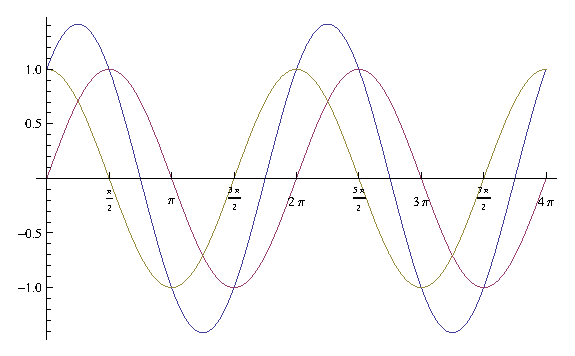
\includegraphics{extraCredit.eps}
        \caption{Extra Credit (all three graphs)}
      \end{figure}
      \end{solution}

    \item Write $f(x)$ as $f(x) = a \cos (bx + c)$
      \begin{solution}
        \[
          f(x) = \sqrt{2} \cos \left( x - \frac{\pi}{4} \right)
        \]
      \end{solution}

  \end{enumerate}

  \ifprintanswers

    \pagebreak

    \section{Section 5.4}
    \begin{description}

      \item[7]
        
        \begin{figure}[H]
          \centering
          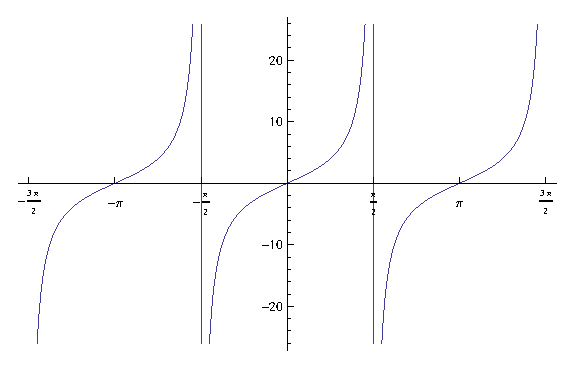
\includegraphics[scale=0.9]{exercise07.eps}

          $f(x) = 4 \tan x$; period: $\pi$

        \end{figure}

      \item[8]
        \begin{figure}[H]
          \centering
          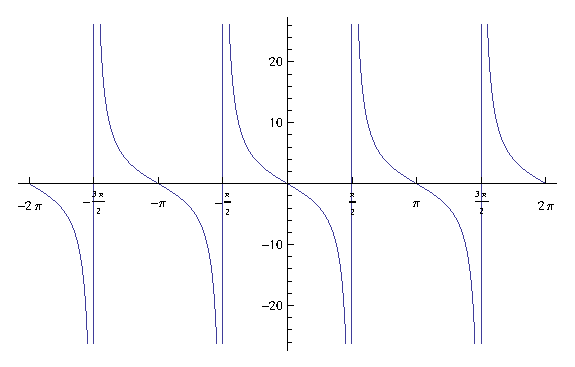
\includegraphics[scale=0.9]{exercise08.eps}

          $f(x) = -4 \tan x$; period: $\pi$
        \end{figure}

      \item[11]
        \begin{figure}[H]
          \centering
          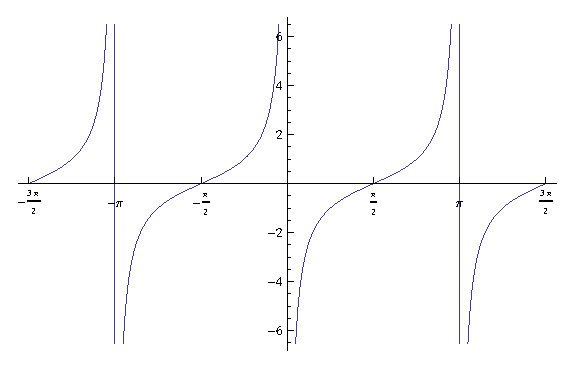
\includegraphics[scale=0.9]{exercise11.eps}

          $f(x) = - \cot x$; period: $\pi$
        \end{figure}

      \item[12]
        \begin{figure}[H]
          \centering
          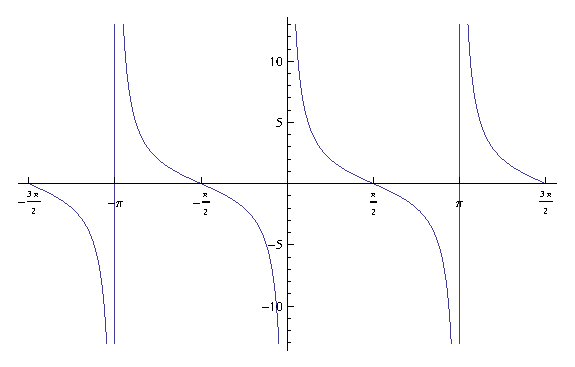
\includegraphics[scale=0.9]{exercise12.eps}

          $f(x) = 2 \cot x$; period: $\pi$
        \end{figure}

      \item[13]
        \begin{figure}[H]
          \centering
          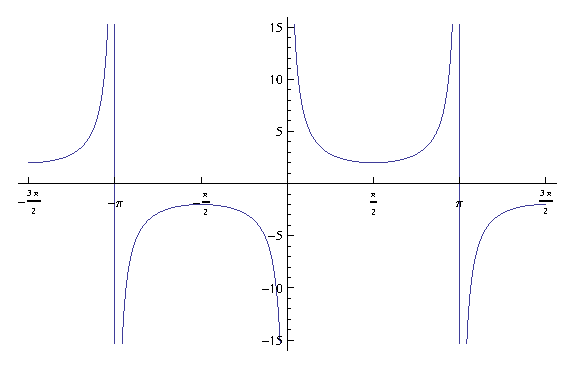
\includegraphics[scale=0.9]{exercise13.eps}

          $f(x) = 2 \csc x$; period: $2 \pi$
        \end{figure}

      \item[14]
        \begin{figure}[H]
          \centering
          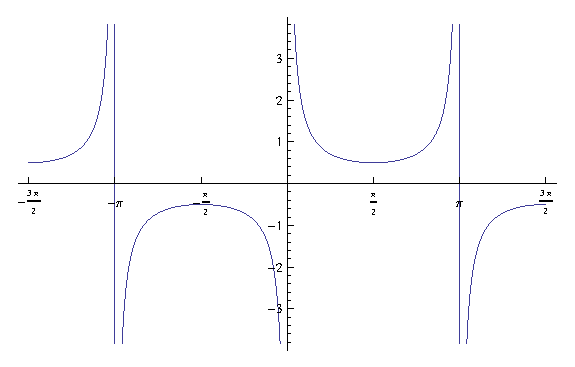
\includegraphics[scale=0.9]{exercise14.eps}

          $f(x) = \frac{1}{2} \csc x$; period: $2 \pi$
        \end{figure}

      \item[15]
        \begin{figure}[H]
          \centering
          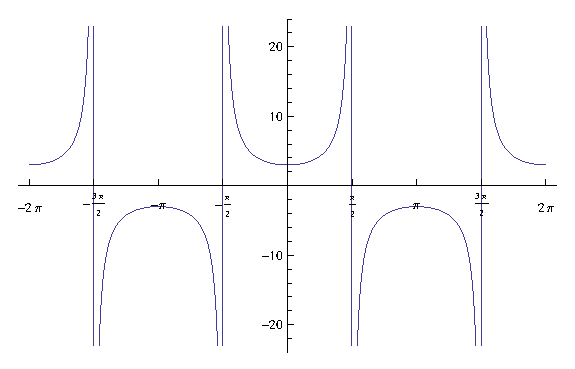
\includegraphics[scale=0.9]{exercise15.eps}

          $f(x) = 3 \sec x$; period: $2 \pi$
        \end{figure}

      \item[16]
        \begin{figure}[H]
          \centering
          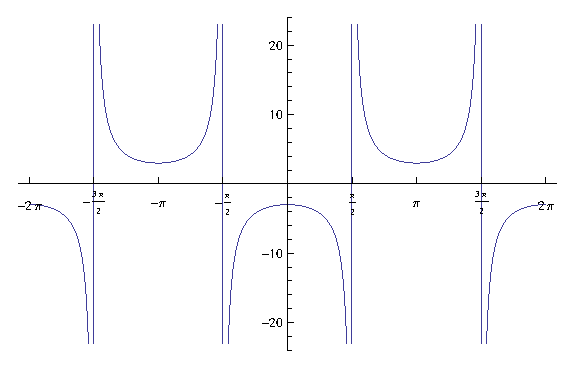
\includegraphics[scale=0.9]{exercise16.eps}

          $f(x) = -3 \sec x$; period: $2 \pi$
        \end{figure}

      \item[17]
        \begin{figure}[H]
          \centering
          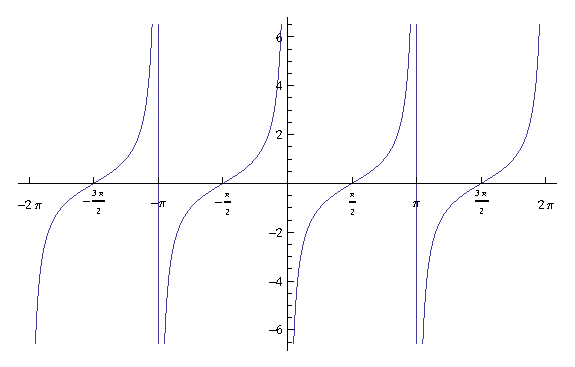
\includegraphics[scale=0.9]{exercise17.eps}

          $f(x) = \tan \left( x + \frac{\pi}{2} \right)$; period: $\pi$
        \end{figure}

      \item[18]
        \begin{figure}[H]
          \centering
          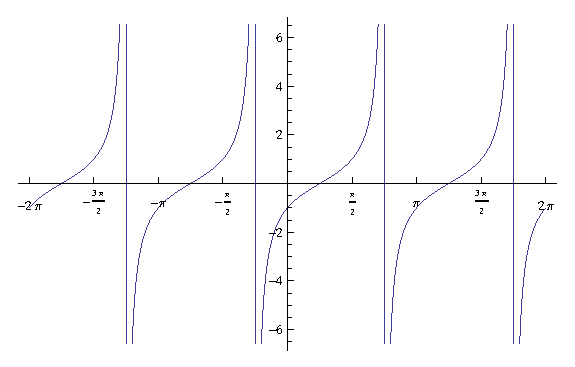
\includegraphics[scale=0.9]{exercise18.eps}

          $f(x) = \tan \left( x - \frac{\pi}{4} \right)$; period: $\pi$
        \end{figure}

      \item[19]
        \begin{figure}[H]
          \centering
          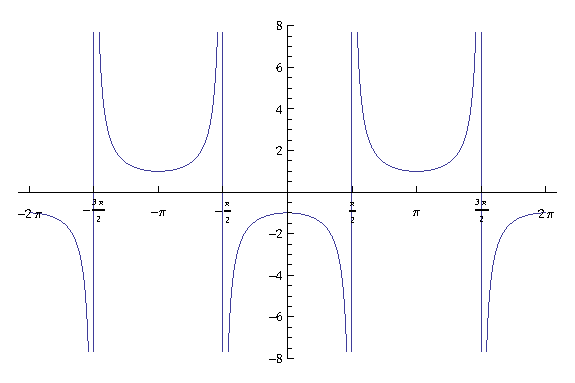
\includegraphics[scale=0.9]{exercise19.eps}

          $f(x) = \csc \left( x - \frac{\pi}{2} \right)$; period: $2 \pi$
        \end{figure}

      \item[20]
        \begin{figure}[H]
          \centering
          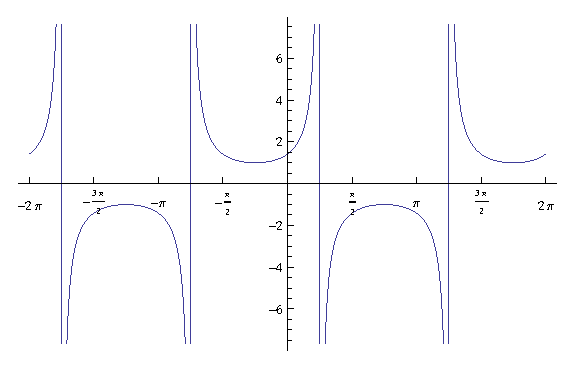
\includegraphics[scale=0.9]{exercise20.eps}

          $f(x) = \sec \left( x + \frac{\pi}{4} \right)$; period: $2 \pi$
        \end{figure}

      \item[25]
        \begin{figure}[H]
          \centering
          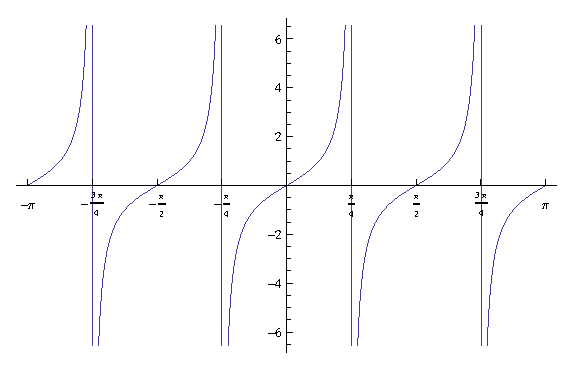
\includegraphics[scale=0.9]{exercise25.eps}

          $f(x) = \tan 2x$; period: $\frac{\pi}{2}$
        \end{figure}

      \item[26]
        \begin{figure}[H]
          \centering
          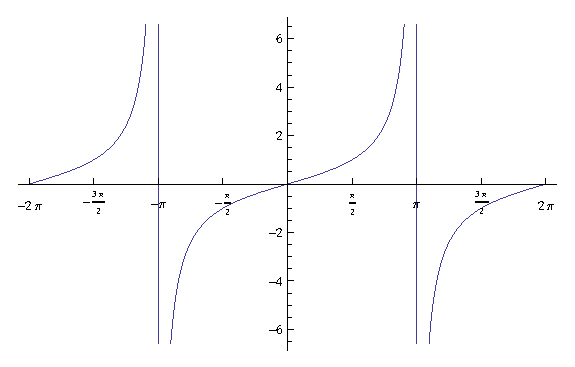
\includegraphics[scale=0.9]{exercise26.eps}

          $f(x) = \tan \frac{1}{2} x $; period: $2 \pi$
        \end{figure}

      \item[27]
        \begin{figure}[H]
          \centering
          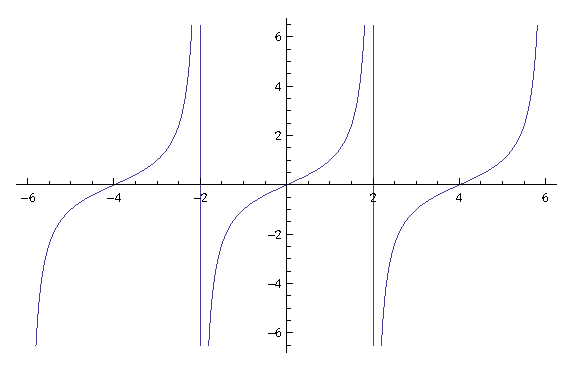
\includegraphics[scale=0.9]{exercise27.eps}

          $f(x) = \tan \frac{\pi}{4} x $; period: $4$
        \end{figure}

      \item[28]
        \begin{figure}[H]
          \centering
          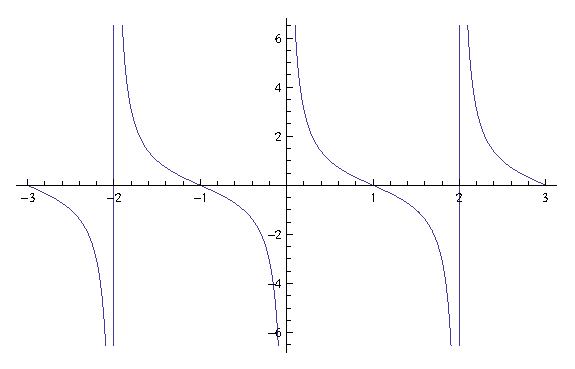
\includegraphics[scale=0.9]{exercise28.eps}

          $f(x) = \cot \frac{\pi}{2} x $; period: $2$
        \end{figure}

      \item[29]
        \begin{figure}[H]
          \centering
          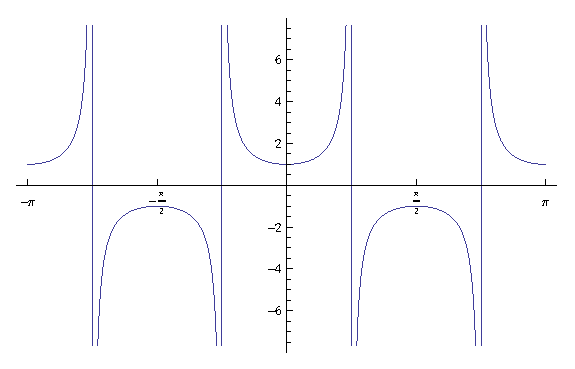
\includegraphics[scale=0.9]{exercise29.eps}

          $f(x) = \sec 2x $; period: $\pi$
        \end{figure}

      \item[30]
        \begin{figure}[H]
          \centering
          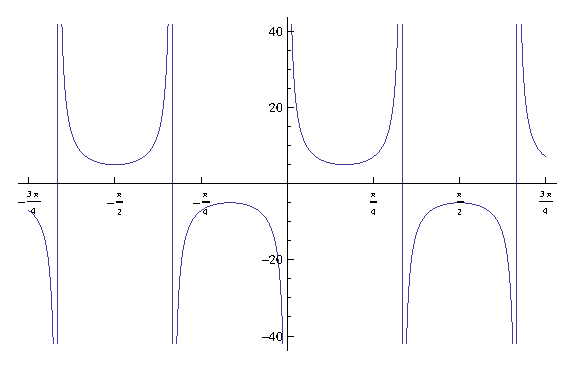
\includegraphics[scale=0.9]{exercise30.eps}

          $f(x) = 5 \csc 3x $; period: $\frac{2 \pi}{3}$
        \end{figure}

      \item[37]
        \begin{figure}[H]
          \centering
          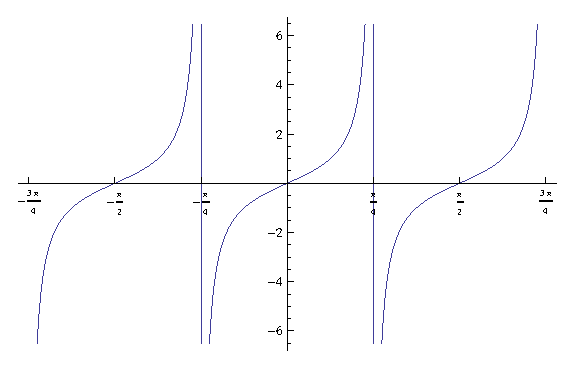
\includegraphics[scale=0.9]{exercise37.eps}

          $f(x) = \tan 2 \left( x + \frac{\pi}{2} \right) $; period: $\frac{\pi}{2}$
        \end{figure}

      \item[38]
        \begin{figure}[H]
          \centering
          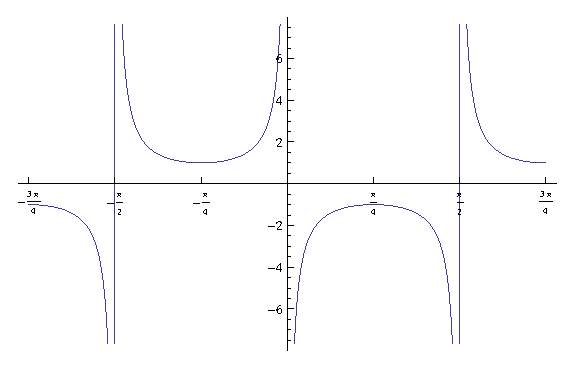
\includegraphics[scale=0.9]{exercise38.eps}

          $f(x) = \csc 2 \left( x + \frac{\pi}{2} \right) $; period: $\pi$
        \end{figure}

      \item[39]
        \begin{figure}[H]
          \centering
          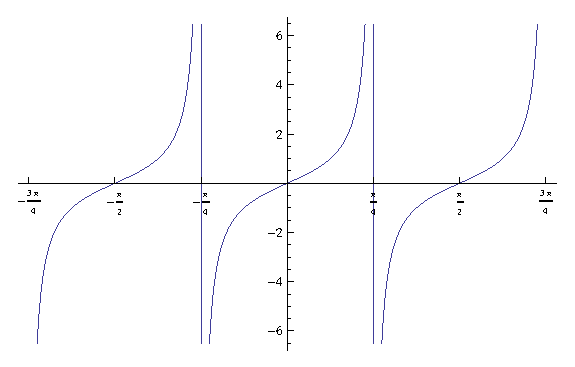
\includegraphics[scale=0.9]{exercise39.eps}

          $f(x) = \tan 2 (x - \pi) $; period: $\frac{\pi}{2}$
        \end{figure}

      \item[40]
        \begin{figure}[H]
          \centering
          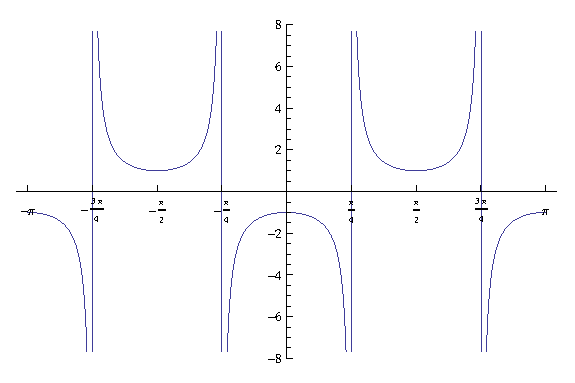
\includegraphics[scale=0.9]{exercise40.eps}

          $f(x) = \sec 2 \left( x - \frac{\pi}{2} \right) $; period: $\pi$
        \end{figure}

      \item[41]  

        \begin{figure}[H]
          \centering
          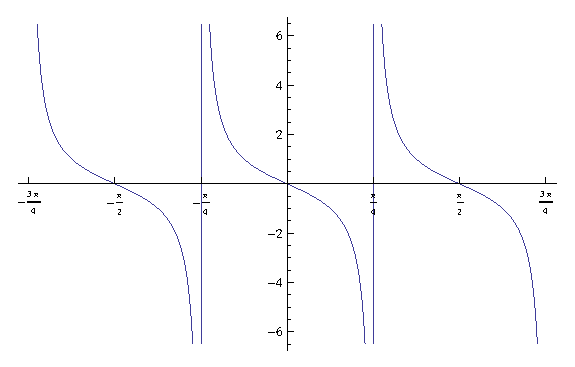
\includegraphics[scale=0.9]{exercise41.eps}

          $f(x) = \cot \left( 2x - \frac{\pi}{2} \right) = \cot 2 \left( x - \frac{\pi}{4} \right)$
        \end{figure}

      \item[47] 

        \begin{figure}[H]
          \centering
          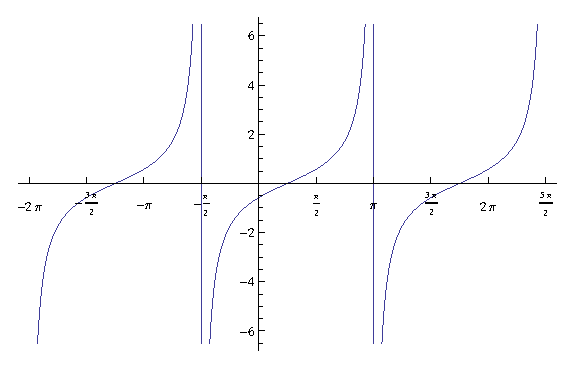
\includegraphics[scale=0.9]{exercise47.eps}

          $f(x) = \tan \left( \frac{2}{3} x - \frac{\pi}{6} \right) = \tan \frac{2}{3} \left( x - \frac{\pi}{4} \right)$
        \end{figure}

      \item[48] 

        \begin{figure}[H]
          \centering
          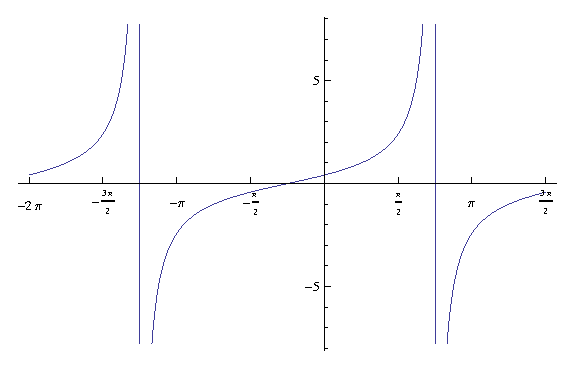
\includegraphics[scale=0.9]{exercise48.eps}

          $f(x) = \tan \left( \frac{2}{3} x - \frac{\pi}{6} \right) = \tan \frac{2}{3} \left( x - \frac{\pi}{4} \right)$
        \end{figure}

      \item[49]
        \begin{figure}[H]
          \centering
          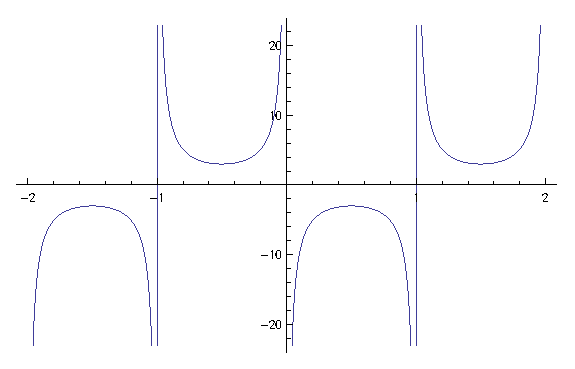
\includegraphics[scale=0.9]{exercise49.eps}

          $f(x) = 3 \sec \pi \left( x + \frac{1}{2} \right)$; period: $2$
        \end{figure}

      \item[50]  

        \begin{figure}[H]
          \centering
          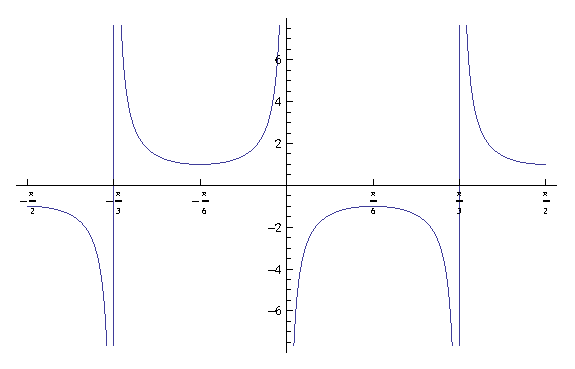
\includegraphics[scale=0.9]{exercise50.eps}

          $f(x) = \sec \left( 3x + \frac{\pi}{2} \right) = \sec 3 \left( x + \frac{\pi}{6} \right)$
        \end{figure}

      \item[55]
        \begin{parts}
          \part
            \begin{align*}
              d(0.15) &\approx 1.5286 \\
              d(0.25) &= 3 \\
              d(0.45) &\approx 18.941 \\
            \end{align*}

          \part
            \begin{figure}[H]
              \centering
              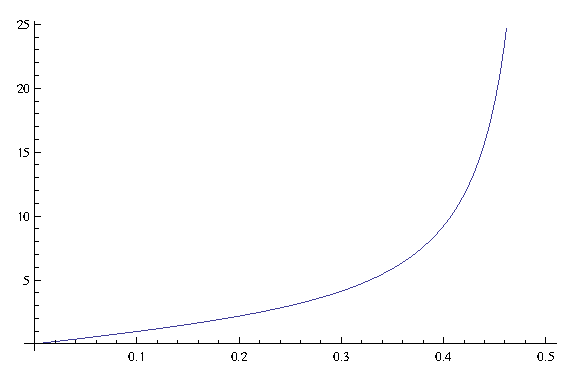
\includegraphics[scale=0.9]{exercise55.eps}

              Exercise 55
            \end{figure}

          \part The distance gets larger as $t$ approaches \sfrac{1}{2}.

        \end{parts}

      \item[56]
        \begin{parts}
          \part
          
            \begin{align*}
              s(2)     &\approx 10.392 \\
              s(6)     &= 0 \\
              s(8)     &\approx 3.4641 \\
              s(11.75) &\approx 91.542 \\
            \end{align*}

          \part
            \begin{figure}[H]
              \centering
              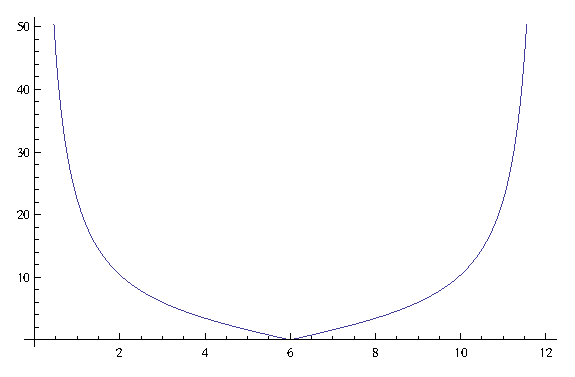
\includegraphics[scale=0.9]{exercise56.eps}
              
              Exercise 56
            \end{figure}

          \part The shadow is 6 feet at 9:00 and 3:00.  This makes sense since this is exactly half way between
          sunrise/sunset and noon if sunrise/sunset is at 6:00.

          \part The shadow gets longer and longer as the sun sets.

        \end{parts}
    \end{description}

  \else
    \vspace{3 cm}
    \begin{quote}
      \begin{em}
        The fool doth think he is wise, but the wise man knows himself to be a fool
      \end{em}
    \end{quote}
    \hspace{1 cm} --William Shakespeare, {\em As You Like It}
  \fi

\end{document}

